En el \fullref{chap:ppa} vimos a \ppaLang{} como un lenguaje, desde el punto de
vista de un usuario. En \fullref{chap:ppa-certifier} abordamos el funcionamiento
interno, que expandimos en \fullref{chap:witness-extraction} con extracción de
testigos. En este capítulo presentamos la herramienta de línea de comandos
\ppaTool{}, que permite procesar programas del lenguaje. Está implementada en Haskell.

\section{Instalación}

Para instalar \ppaTool{} a partir de los fuentes, seguir los siguientes pasos.

\begin{enumerate}
    \item Instalar \href{https://www.haskell.org/}{Haskell}, \href{https://www.haskell.org/cabal/}{Cabal}
    \item Clonar el repositorio de \ppaTool{} o descargarlo \url{https://github.com/mnPanic/tesis}
    \item Instalar la herramienta con cabal
    \begin{minted}{bash}
tesis/ppa:~$ cabal install ppa
    \end{minted}
    \item Verificar la instalación
    \begin{minted}{bash}
tesis/ppa:~$ ppa version
ppa version 0.1.0.0
    \end{minted}
\end{enumerate}

\section{Interfaz y ejemplos}

El ejecutable \ppaTool{} cuenta con dos comandos: \texttt{check} (certificado y
chequeo de programas) y \texttt{extract} (extracción de testigos). En el
repositorio de los fuentes, el directorio \texttt{ppa/doc/examples} contiene
ejemplos de programas. La extensión por convención de programas de \ppaTool{} es \texttt{.ppa}.

\subsection{\texttt{check} - Chequeo de programas}

Permite certificar y chequear programas.

\begin{minted}{bash}
ppa check <in> <args>
\end{minted}

Argumentos:

\begin{itemize}
    \item El primer argumento posicional es el archivo que contiene el programa
    a certificar. Puede ser \texttt{-} para leer de \textit{stdin}.
    \item \texttt{--out}, \texttt{-o} (\textit{opcional}): Path para el archivo
    al cual escribir el certificado (con el sufijo \texttt{\_raw.nk}) o
    \texttt{-} para usar \textit{stdout}.
\end{itemize}


Primero lee, certifica y chequea el programa reportando el resultado. En caso de
haber proporcionado un archivo de output, escribe el certificado de deducción
natural a \texttt{<path>\_raw.nk}.

Ejemplos:

\begin{minted}{bash}
$ ppa check doc/examples/parientes.ppa
Checking... OK!
\end{minted}

\begin{minted}{bash}
$ ppa check doc/examples/parientes.ppa --out out   
Checking... OK!
Writing...
Wrote raw to out_raw.nk
\end{minted}

\subsection{\texttt{extract} - Extracción de testigos}

Permite ejecutar la extracción de testigos.

\begin{minted}{bash}
ppa extract <in> <args>
\end{minted}

Argumentos:

\begin{itemize}
    \item El primer argumento posicional es el archivo de entrada que contiene
    el programa. Puede ser \texttt{-} para leer de \textit{stdin}.
    \item \texttt{--theorem}, \texttt{-t} (\textit{obligatorio}): el nombre del
    teorema para el cual extraer el testigo
    \item \texttt{--terms}, \texttt{ts}: la lista de términos que indica cómo
    instanciar las variables cuantificadas universalmente. Debe contener la
    misma cantidad de términos que variables.
    \item \texttt{--out}, \texttt{-o} (\textit{opcional}): Path para el archivo
    al cual escribir los certificados (con los sufijos \texttt{\_raw.nk} y
    \texttt{.nj}) o \texttt{-} para usar \textit{stdout}.
\end{itemize}

Primero lee y certifica, y chequea el programa. Luego, lo traduce con la
traducción de Friedman, normaliza la demostración e intenta extraer un testigo,
reportando cual fue el testigo extraído y cómo queda el término final con el
testigo y los términos proporcionados para instanciar las variables
cuantificadas universalmente.

Por ejemplo, si tenemos el programa de \namedref{fri:prog:forall}

\begin{minted}{bash}
$ ppa extract doc/listings/extract/forall.ppa --theorem t --terms x
Running program... OK!
Translating... OK!
Checking translated... OK!
Extracted witness: v
of formula: p(x, v)
\end{minted}

Y especificando output,

\begin{minted}{bash}
$ ppa extract doc/listings/extract/forall.ppa --theorem t --terms x -o out
Running program... OK!
Translating... OK!
Writing...
Wrote raw to out_raw.nk
Wrote translated+reduced to out.nj
Checking translated... OK!
Extracted witness: v
of formula: p(x, v) 
\end{minted}

\section{Detalles de implementación}

En esta sección contamos algunos detalles relevantes sobre la implementación,
que deberían permitir navegar los fuentes para ver cómo fue implementado.
Comencemos por la arquitectura de los módulos.

\begin{figure}[h]
    \centering
    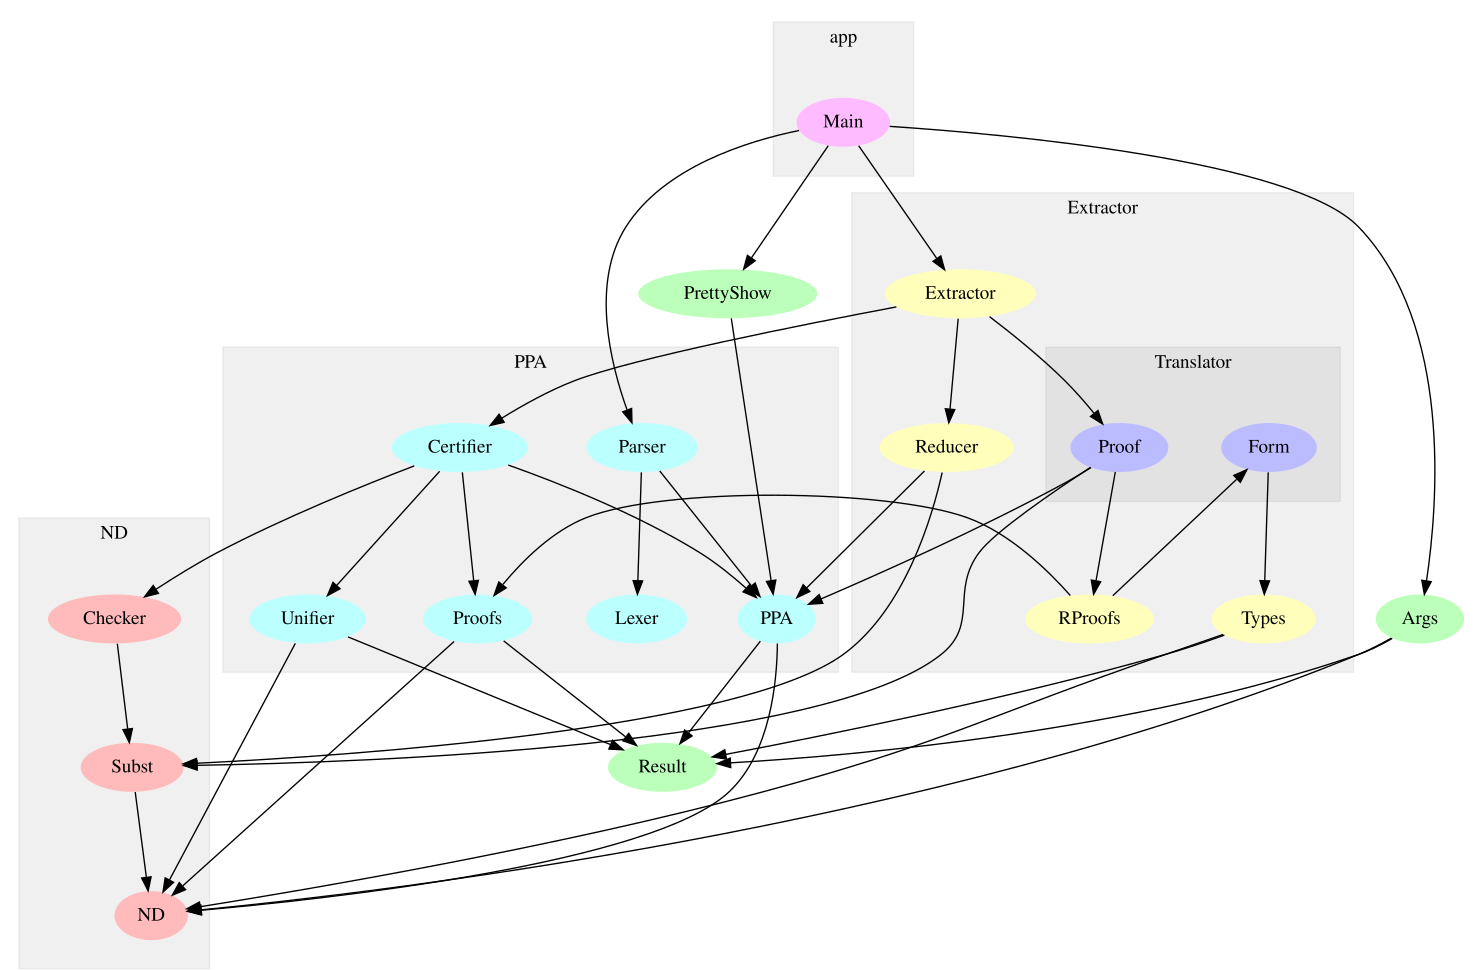
\includegraphics[scale=0.38]{img/modules.png}
    \caption{Grafo de módulos del programa \ppaTool{} generado con \href{https://github.com/yav/graphmod}{\texttt{graphmod}}}
\end{figure}

Los más relevantes son,

\begin{itemize}
    \item \texttt{ND}: Contiene el modelo central de deducción natural usado para los
    certificados. Fórmulas, términos y demostraciones. Tiene 3 sub módulos:
    \texttt{ND.Checker} (chequeador de demostraciones), \texttt{ND.Subst}
    (sustituciones sobre fórmulas y demostraciones) y \texttt{ND.ND} (el modelo
    en si). Ver \fullref{ppa-tool:sec:nd}.
    \item \texttt{PPA}: Contiene la implementación del lenguaje \ppaLang{} por
    sobre deducción natural.
    \begin{itemize}
        \item \texttt{PPA.Parser} y \texttt{PPA.Lexer} son el lexer y el parser
        respectivamente. Ver \fullref{ppa-tool:sec:parser-lexer}.
        \item \texttt{PPA.Certifier} implementa el certificador, que genera
        demostraciones de deducción natural a partir de programas de PPA. Usa
        \texttt{PPA.Unifier} para unificación (usado en eliminación de $\forall$) y \texttt{PPA.Proofs} para
        demostraciones de equivalencias en ND (usado en DNF).
    \end{itemize}
    \item \texttt{Extractor}: Contiene la lógica de extracción de testigos.
    Tiene varios sub módulos
    \begin{itemize}
        \item \texttt{Extractor.Translator} implementa la traducción de Friedman
        en sus dos sub-módulos, \texttt{Extractor.Translator.Proof} para
        demostraciones y\\\texttt{Extractor.Translator.Form} para fórmulas.
        \item \texttt{Extractor.Reducer} implementa la normalización.
        \item \texttt{Extractor.Extractor} combina todo lo anterior para hacer
        la extracción de testigos de principio a fin, certificando, traduciendo
        y reduciendo. Usa \\\texttt{Extractor.RProofs} que es análogo a
        \texttt{PPA.Proofs} e implementa los lemas necesarios sobre
        demostraciones intuicionistas con negación relativizada.
    \end{itemize}
\end{itemize}


\subsection{Parser y Lexer}
\label{ppa-tool:sec:parser-lexer}

Una parte esencial de \ppaTool{} es el compilador, que permite tomar un programa
desde un archivo de texto y llevarlo a una representación estructurada, como un
un tipo abstracto de datos, para el uso en el resto del programa. Se implementa
en dos etapas.

\begin{itemize}
    \item La primera es el análisis léxico o \textit{lexer}, que convierte el
    texto plano en una lista de \textit{lexemas} o \textit{tokens}. Se puede
    implementar con expresiones regulares.
    \item Una vez que el programa ya fue convertido en \textit{lexemas}, es
    procesado por el parser, que interpreta las estructuras sintácticas del
    lenguaje. Puede generar una representación intermedia como un tipo abstracto
    de datos.
\end{itemize}

Para el parsing en general hay dos caminos bien conocidos. O bien hacerlo a mano
con alguna biblioteca de \textit{parser combinators} como
\href{https://hackage.haskell.org/package/parsec}{parsec}, o usar un
\textit{parser generator}: un programa que genere un parser automáticamente a
partir de una gramática en algún formato como EBNF. Nosotros decidimos, por
familiaridad con el proceso, usar un parser generator. Los más conocidos
históricamente son Lex (para el lexer) y Yacc (para el parser, \textit{yet
another compiler compiler}). En Haskell existen dos paquetes análogos: \href{https://hackage.haskell.org/package/alex}{Alex} para el
lexer y \href{https://hackage.haskell.org/package/happy}{Happy} para el parser.
Estos generan un lexer a partir de expresiones regulares y un parser
respectivamente a partir de una gramática en un formato similar a EBNF.

En la \namedref{ppa-tool:fig:lexer} se puede ver un extracto del archivo de
input de Alex y en \namedref{ppa-tool:fig:parser} uno del de Happy de
\ppaTool{}. La implementación del parser solo construye términos de programas
(definidos en \texttt{PPA.PPA}) y fórmulas (\texttt{ND.ND}) a partir de los
cuales el programa opera.

\begin{figure}[p]
    \begin{minted}{text}
tokens :-
    $white+                         ;
    "//".*                          ; -- comments
    "/*"(.|(\r\n|\r|\n))*"*/"       ; -- block comments
    \.              { literal TokenDot }
    \,              { literal TokenComma }
    \&              { literal TokenAnd }
    \|              { literal TokenOr }
    true            { literal TokenTrue }
    false           { literal TokenFalse }
    \-\>            { literal TokenImp }
    \<\-\>          { literal TokenIff }
    \~              { literal TokenNot }
    exists          { literal TokenExists }
    forall          { literal TokenForall }
    \(              { literal TokenParenOpen }
    \)              { literal TokenParenClose }
    axiom           { literal TokenAxiom }
    theorem         { literal TokenTheorem }
    proof           { literal TokenProof }
    end             { literal TokenEnd }
    \;              { literal TokenSemicolon }
    \:              { literal TokenDoubleColon }
    suppose         { literal TokenSuppose }
    thus            { literal TokenThus }
    hence           { literal TokenHence }
    have            { literal TokenHave }
    then            { literal TokenThen }
    by              { literal TokenBy }
    equivalently    { literal TokenEquivalently }
    claim           { literal TokenClaim }
    cases           { literal TokenCases }
    case            { literal TokenCase }
    take            { literal TokenTake }
    \:\=            { literal TokenAssign }
    st              { literal TokenSuchThat }
    consider        { literal TokenConsider }
    let             { literal TokenLet }

    \"[^\"]*\"          { lex (TokenQuotedName . firstLast) }

    (\_|[A-Z])[a-zA-Z0-9\_\-]*(\')*                     { lex TokenVar }
    [a-zA-Z0-9\_\-\?!#\$\%\*\+\<\>\=\?\@\^]+(\')*       { lex TokenId }
    \end{minted}
    \caption{Extracto del lexer de \ppaTool{}}
    \label{ppa-tool:fig:lexer}
\end{figure}

\begin{figure}[p]
    \centering
    \begin{minted}{text}
%token
    -- Enumeración de tokens del lexer

Prog    : Declarations

Declarations : Declaration Declarations
                | Declaration

Declaration : Axiom
            | Theorem

Axiom : axiom Name ':' Form

Theorem : theorem Name ':' Form proof Proof end

Proof   : ProofStep Proof
        | {- empty -}

ProofStep : suppose Name ':' Form
            | thus Form OptionalBy
            | hence Form OptionalBy
            | have Name ':' Form OptionalBy
            | then Name ':' Form OptionalBy
            | equivalently Form
            | claim Name ':' Form proof Proof end
            | cases OptionalBy Cases end
            | take var ':=' Term
            | let var
            | consider var st Name ':' Form by Justification

Cases   : Case Cases
        | {- empty -}

Case    : case Form Proof
        | case Name ':' Form Proof

OptionalBy : by Justification
OptionalBy : {- empty -}

Justification : Name ',' Justification
                | Name

Name    : id
        | name

    \end{minted}
    \caption{Extracto del parser de \ppaTool{} (programas)}
    \label{ppa-tool:fig:parser}
\end{figure}

\begin{figure}[p]
    \begin{minted}{text}
-- Resolución automática de conflictos shift/reduce
%right exists forall dot
%right imp iff
%left and or
%nonassoc not
%%

Form    : id TermArgs
        | Form and Form
        | Form or Form
        | Form imp Form
        | Form iff Form
        | not Form
        | exists var dot Form
        | forall var dot Form
        | true
        | false
        | '(' Form ')'

Term    : var
        | id TermArgs

TermArgs : {- empty -}
            | '(' Terms ')'

Terms   : Term
        | Term ',' Terms
    \end{minted}
    \caption{Extracto del parser de \ppaTool{} (lógica de primer orden)}
    \label{ppa-tool:fig:parser-forms}
\end{figure}

\subsection{Modelado de deducción natural}
\label{ppa-tool:sec:nd}

La parte más interesante del modelado son las demostraciones de deducción
natural, que se pueden ver en la \namedref{ppa-tool:fig:nd-proofs}. Una
demostración está compuesta por la aplicación recursiva de reglas de inferencia,
y su modelo omite todos los detalles que se pueden inferir durante su chequeo.
De esa forma las demostraciones son más fáciles de escribir y generar, al costo
de ser un poco más costosas de leer por un humano, cosa que de todas formas no
deberíamos hacer. Por ejemplo, la introducción de la implicación, \ruleImpI{},
modelada por \texttt{PImpI} no especifica cuál es la implicación que se está
introduciendo, dado que durante el chequeo debería ser la fórmula actual a
demostrar. Tampoco se explicita en cada regla, cual es el contexto de
demostración. Se genera de forma dinámica.

\begin{figure}[p]
    \begin{multicols}{2}
    \begin{minted}{haskell}
    type VarId = String
    type FunId = String
    type PredId = String
    type HypId = String
    
    data Term
        = TVar VarId
        | TMetavar Metavar
        | TFun FunId [Term]
    
    data Form
        = FPred PredId [Term]
        | FAnd Form Form
        | FOr Form Form
        | FImp Form Form
        | FNot Form
        | FTrue
        | FFalse
        | FForall VarId Form
        | FExists VarId Form
    \end{minted}
    \end{multicols}
    \caption{Modelado de fórmulas y términos de LPO}
    \end{figure}
    

\begin{figure}[p]
\begin{multicols}{2}
\begin{minted}{haskell}
data Proof =
    | PAx HypId
    | PAndI
        { proofLeft :: Proof
        , proofRight :: Proof
        }
    | PAndE1
        { right :: Form
        , proofAnd :: Proof
        }
    | PAndE2
        { left :: Form
        , proofAnd :: Proof
        }
    | POrI1
        { proofLeft :: Proof
        }
    | POrI2
        { proofRight :: Proof
        }
    | POrE
        { left :: Form
        , right :: Form
        , proofOr :: Proof
        , hypLeft :: HypId
        , proofAssumingLeft :: Proof
        , hypRight :: HypId
        , proofAssumingRight :: Proof
        }
    | PImpI
        { hypAntecedent :: HypId
        , proofConsequent :: Proof
        }
    | PImpE
        { antecedent :: Form
        , proofImp :: Proof
        , proofAntecedent :: Proof
        }
    | PNotI
        { hyp :: HypId
        , proofBot :: Proof
        }
    | PNotE
        { form :: Form
        , proofNotForm :: Proof
        , proofForm :: Proof
        }
    | PTrueI
    | PFalseE
        { proofBot :: Proof
        }
    | PLEM
    | PForallI
        { newVar :: VarId
        , proofForm :: Proof
        }
    | PForallE
        { var :: VarId
        , form :: Form
        , proofForall :: Proof
        , termReplace :: Term
        }
    | PExistsI
        { inst :: Term
        , proofFormWithInst :: Proof
        }
    | PExistsE
        { var :: VarId
        , form :: Form
        , proofExists :: Proof
        , hyp :: HypId
        , proofAssuming :: Proof
        }
\end{minted}        
\end{multicols}
\caption{Modelado de reglas de inferencia para demostraciones}
\label{ppa-tool:fig:nd-proofs}
\end{figure}